\section{Spur \& Helical Gear Design}

\newthought{Now we have selected our gear ratio} and level of damping within our system, we can start to look at the design of the gearbox that will be used to generate the ratio. In this exercise we will look at creating a multi-stage spur or helical gearbox and it will good for you to discuss the affordances of each in your report before selecting one type to carry forward.

This section describes some common types of gear as well as providing some gear design guidelines that you will be using to create your multi-stage gearbox. The result will be a spreadsheet of all the stages of your gearbox with a breakdown of the forces as well as an engineering schematic of your gearbox layout.

\subsection{Gear Types}

% https://s.hswstatic.com/gif/gear-spur.jpg
\begin{marginfigure}[10em]
  \centering
  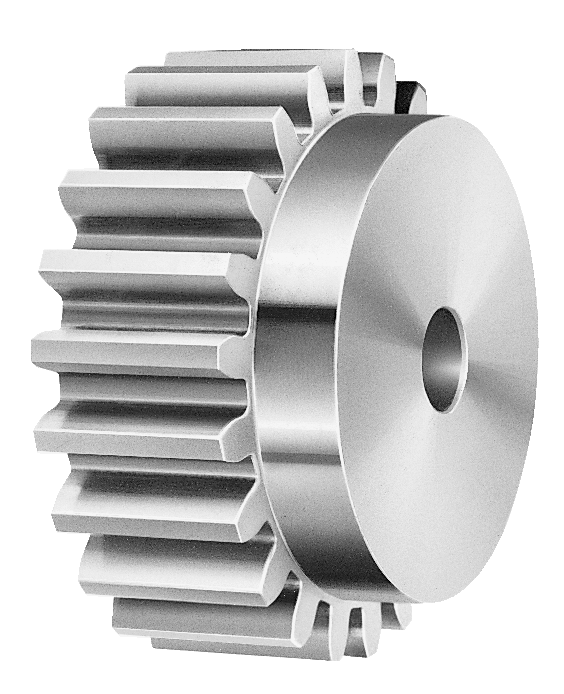
\includegraphics[width=0.4\textwidth]{figs/spur.png}
  \caption{Spur Gear}
\end{marginfigure} 
Spur gears are one of the most common types of gear in mechanical systems. 
The teeth often have a involute profile to achieve a constant drive ratio between the gears. Gears have to be fitted on parallel shafts. An affordance of the design is that no axial load is produced by the mating of the teeth. They are typically used in low/medium speed environments where the pitch line velocity is $<\SI{25}{\metre\per\second}$~\footnote{rule of thumb}. Applications include engines, power plants, fuel pumps, washing machines and rack \& pinion mechanisms.

They have the ability to transmit large amounts of power with designs known to cope with \SI{50,000}{\kilo\watt}. They are very reliable, provide a constant velocity ratio and are simple to manufacture. However, initial contact between teeth occurs across the entire tooth face, which leads to higher stresses on the gear teeth. They can also become very noisy at high speeds.

% https://s.hswstatic.com/gif/gear-helical1.jpg
\begin{marginfigure}[12em]
  \centering
  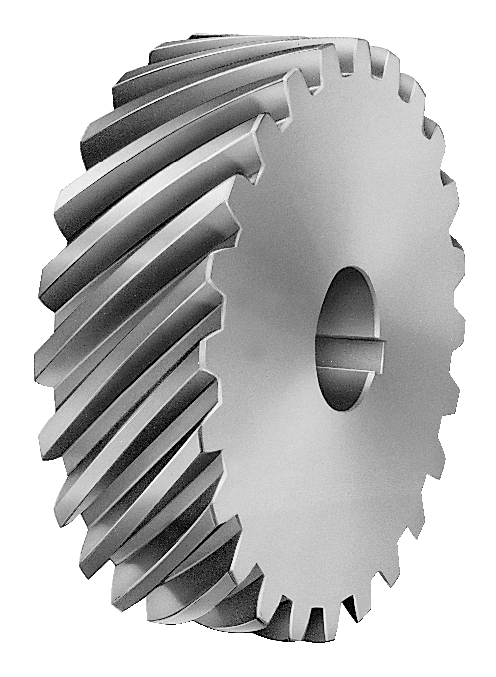
\includegraphics[width=0.4\textwidth]{figs/helical.png}
  \caption{Helical Gear}
\end{marginfigure} 
Helical gears differ from spur gears by introducing an angle to the leading edge of the gear teeth and the axis of rotation. This leads to a curved gear that is a segment of a helix. The angling of the gear enables smoother running due to a less aggressive engagement of the gear faces. This also leads to a reduction in noise when running at high speeds and the ability to carry more load per width of gear.

Thus, helical gears are often used in higher speed environments $>\SI{25}{\metre\per\second}$ and environments where noise abatement is an issue. Applications include elevators and conveyors. 

However, the angling of the gears leads to the introduction of an axial force component, which requires reaction by thrust bearings along the shafts. In addition, there is greater heat generation through the mating of gears and this in turn, leads to a reduction in efficiency when compared to spur.

\begin{marginfigure}
  \centering
  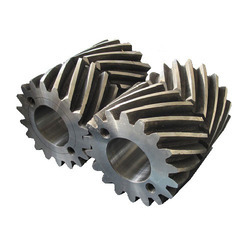
\includegraphics[width=0.6\textwidth]{figs/herringbone-gear.jpg}
  \caption{Double Helical (Herringbone)}
\end{marginfigure}
Herringbone gears are effectively two helical gears positioned back to back with one another and are used in a range of application including 3D printers and heavy machinery. They have the same affordance of helical gears of providing a smoother motion and have a greater resistance to operation disruption if teeth start to become damaged and/or missing. The main challenge with herringbone gears is that they are difficult to manufacture, which leads to the gear sets costing more than their helical/spur counterparts.

% http://www.aero-news.net/images/content/commav/2008/PW-Geared-Turbofan-0708b.jpg
\begin{marginfigure}
  \centering
  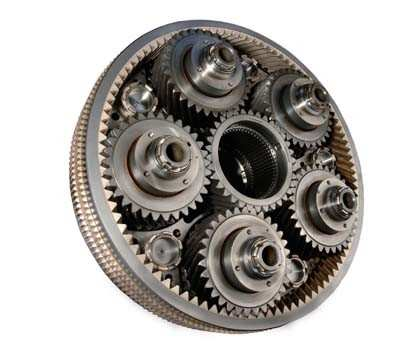
\includegraphics[width=0.8\textwidth]{figs/planetary-gear.jpg}
  \caption{Epicyclic}
\end{marginfigure}
Epicyclic gears provide higher efficiency and power dense solutions to transferring power. They are also highly accurate and enable high gear ratios to be attained per area than that of spur and helical. They also allow in-line input-output shafts.

Applications include lathes, hoists, pulley blocks, watches, automatic transmissions, turbofans and hybrid vehicles. The main challenges in designing epicyclic gears are there loud operation and the high-level of accuracy that needs to be attained between the various gears to ensure the forces are distributed evenly.

% http://www.linngear.com/wp-content/uploads/2012/10/34.png
\begin{marginfigure}
  \centering
  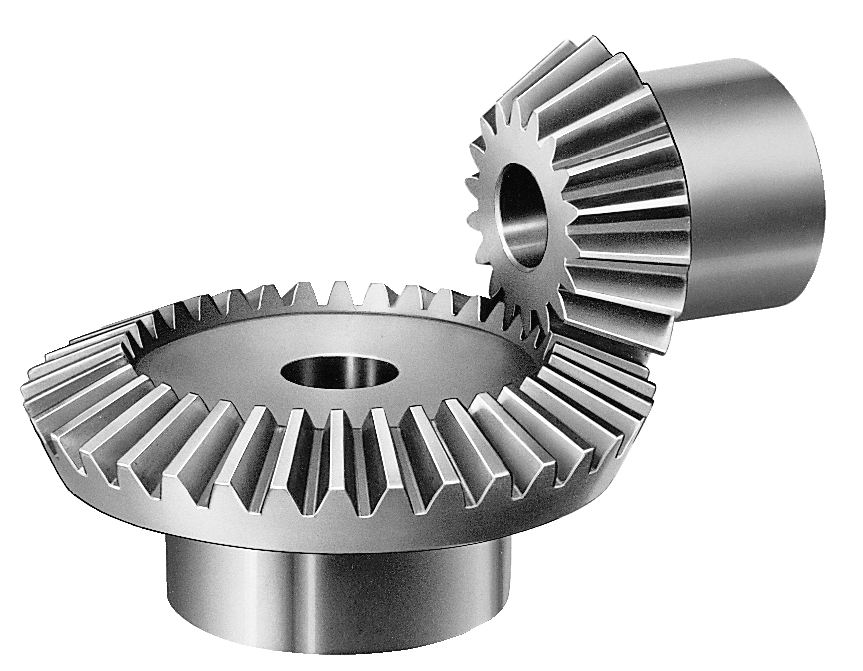
\includegraphics[width=0.8\textwidth]{figs/bevel.png}
  \caption{Bevel}
\end{marginfigure}
Bevel gears are very useful when one wants to change the direction of the power transmission and are applied in differential drives in vehicles, hand drills and assembly machinery. Challenges are in the manufacture of the these components to gain the accuracy required and in mounting the gears in order to provide even contact across the cycle. Bevel gears can have different teeth profiles including involute, spiral and hypoid.

%http://zentexind.com/wp/wp-content/uploads/2016/09/worm-worm-wheel-500x500.jpg
\begin{marginfigure}
  \centering
  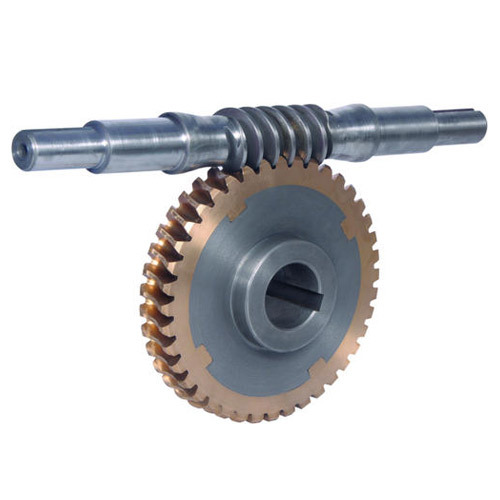
\includegraphics[width=0.8\textwidth]{figs/worm.jpg}
  \caption{Worm \& Wheel}
\end{marginfigure}
The worm \& wheel also enables a \ang{90} torque transfer and provide a near silent and smooth operation. A particular advantage of the worm \& wheel is that they are self-locking and are often used to introduce safety within a system. Application include elevators, hoists, packaging equipment, rock crushers and tuning instruments. They are also able to achieve high-velocity ratios within a single-stage and can absorb shock loading.

Challenges in designing worm \& wheel systems are that they are typically more expensive to manufacture and have much greater power lower losses. This is due to the greater level of heat generation from the multiple teeth in contact between worm \& wheel.

\subsection{Spur \& Helical Gear Guidelines}

Adapted From the Mechanical Design Data Manual.~\cite{MechanicalDesignDataManual2000}

\subsubsection{Introduction}

There are many types of gears used in engineering as set out in Australian Standard AS2075 --- Glossary of Terms and Notations for Gears. Some of the types encountered include:

\begin{itemize}
  \item spur
  \item helical
  \item double helical (herringbone)
  \item bevel
  \item hypoid
  \item worm
\end{itemize}

Two gears in mesh are called a gear pair. Normally gears mesh externally but sometimes the mesh may be internal, that is, one of the gears has the teeth cut internally. The smaller gear of a pair is called the pinion whereas the larger is called the wheel. In a pair of gears, the gear transmitting input torque and power is called the driver whereas the gear transmitting output torque and power is known as the driven. Normally in mechanical power transmission, the driver is the pinion so the wheel rotates at a slower speed than the pinion, that is, there is a reduction in speed through the gear pair. (You might like to discuss the reason why this is so).

Usually gears are cylindrical but other forms are possible of which the most common is the rack and pinion. Here the wheel is flat (of infinite diameter) and is known as a rack.

When more than two gears are in continuous mesh, this is known as a gear train. There are several types of gear train used in mechanical power transmission, including simple, compound and planetary. These are illustrated in Figure~\ref{fig-1}.

\begin{figure}[h!]
  \center
  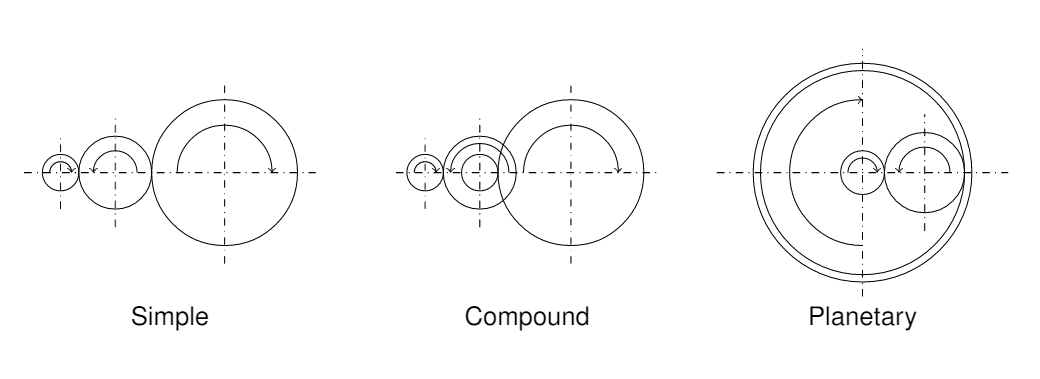
\includegraphics[width=\textwidth]{figs/gear-trains.png}
  \caption{Gear Trains}
  \label{fig-1}
\end{figure}

In the case of the simple gear train, the intermediate gear (or gears) are known as \emph{idler} gears because they do not change the ratio between the driven and driver gears. (You might like to discuss the purpose of idler gears).

Of the various types of gears used in engineering, the most common are spur and helical gears. These are illustrated in \cref{fig-2}.

Spur\marginnote{Spur} gears have the teeth cur parallel to the axis of the shaft.

Helical\marginnote{Helical} gears have the teeth cut at an angle to the axis of the shaft. The angle is called the helix angle, $\alpha$ and is usually about \ang{20} for single helical gears or about 30-\ang{35} for double helical (herringbone) gears.\marginnote[-0.5cm]{\it Note: With a helical gear pair, one helix must be right-hand and the other left-hand.}

\begin{figure}[h!]
  \center
  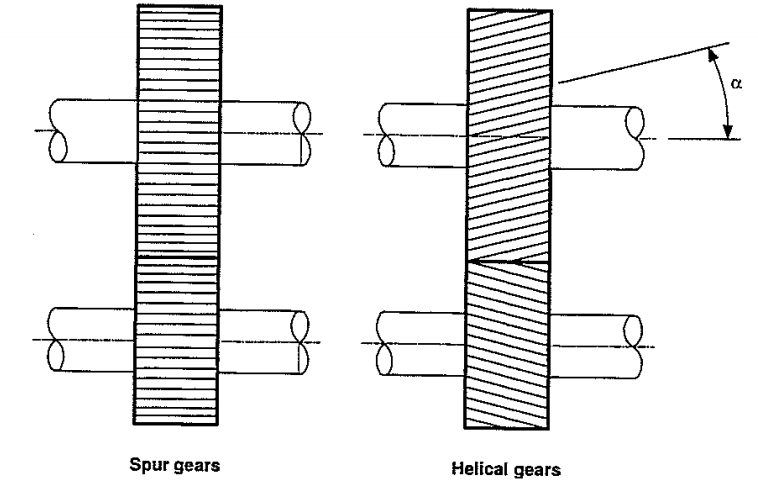
\includegraphics[width=0.9\textwidth]{figs/spur-helical.png}
  \caption{Spur and helical gears}
  \label{fig-2}
\end{figure}

For\marginnote{Velocity Ratio (VR)} all gears other than the worm and wheel, the velocity ratio of a gear pair is the ratio of the number of teeth in each gear. For example, if a 20 tooth pinion meshes with a 40 tooth wheel, the velocity ratio is:

\begin{equation}
  \text{VR} = \frac{40}{20} = 2
\end{equation}

In the case of a compound gear train, the overall velocity ratio is the multiplication of the velocity ratio of each gear pair. If in the above example, the wheel had a 20 tooth pinion attached to it, that meshed with a 60 tooth wheel, the overall velocity ratio is:

\begin{equation}
  \text{VR} = \frac{40}{20} \times \frac{60}{20} = 2 \times 3 = 6
\end{equation}

In the case of a worm and wheel, the velocity ratio is the number of teeth in the wheel divided by the number of starts in the worm. So if a 12 start worm meshed with a 61 tooth wheel, the velocity ratio is:

\begin{equation}
  \text{VR} = \frac{61}{12} = 5.083
\end{equation}

It\marginnote{Number of Teeth} is impractical to have gears with too few teeth (just try and draw a gear with say 3 teeth). To get a reasonable tooth profile without undercutting and with a smooth transfer of power from pinion to wheel, a rule-of-thumb is that spur gears should have at least 17 teeth on the pinion and helical gears (\ang{20} helix angle) should have at least 14 teeth on the pinion.

For maximum life with meshing gears it is desirable to distribute the wear uniformly amongst all teeth, that is not to have the same teeth in mesh for every revolution of the wheel. The best situation possible is that the same teeth mesh together again only after the pinion revolutions equals the number of teeth in the wheel. This is also known as having all the teeth hunting. For example if there are 40 teeth in the wheel, the best possible situation is that re-meshing of the same teeth occurs only after the pinion has made 40 revolutions. The condition for this is that the velocity ratio cannot be reduced to a simpler ratio, that is, there is no common factor between the number of teeth in the pinion and the number of teeth in the gear.

Some possible combinations are given in Table \ref{tbl-1}.

\begin{table}
  \caption{Pinion and wheel combinations}
  \label{tbl-1}
  \center
  \begin{tabular}{p{0.3\textwidth} p{0.3\textwidth} p{0.3\textwidth}}
    \toprule
    Teeth in Pinion & Teeth in Wheel & Revolutions of the pinion when cycle repeats \\
    \midrule
    18 & 38 & 19 \\
    19 & 38 & 2 \\
    20 & 38 & 19 \\
    21 & 38 & 38 \\
    18 & 40 & 20 \\
    19 & 40 & 20 \\
    20 & 40 & 2 \\
    21 & 40 & 40 \\
    \bottomrule
  \end{tabular}
\end{table}

It can be seen therefore, that there can be a huge difference in the way wear will be distributed for approximately the same velocity ratio. However, in practice, exact velocity ratios are often needed (for example, for a camshaft) and in such cases, hunting teeth cannot be provided.

For\marginnote{Limiting Velocity Ratio} a worm-wheel gear pair, the smallest velocity ratio obtainable in practice is about 5. For all other gear pairs, the smallest ratio is 1. There is no theoretical upper limit to the velocity ratio, however high velocity ratios are undesirable because of the large number of teeth that need to be cut in the wheel. This makes accurate machining difficult (if not impossible) and requires large centre distances which are also not usually desirable.

For example, consider a velocity ratio of 125 obtained with single pair of spur gears. With a pinion of 17 teeth and PCD \SI{17}{\milli\metre}, the wheel would require 2125 teeth and a PCD of \SI{2125}{\milli\metre}! The total number of teeth to be cut is 2142!

The same velocity ratio can be obtained with a compound gear train with 3 pairs of gears in mesh, each with a velocity ratio of 5. Then the total number of teeth that need to be cut is 306 (7 times less) and the maximum wheel PCD is only \SI{85}{\milli\metre}.

Rule-of-thumb limits for a gear pair are given in \cref{tbl-2}.

\begin{table}[h]
  \caption{Rule-of-thumb VR limits for a gear pair}
  \label{tbl-2}
  \center
  \begin{tabular}{p{0.3\textwidth} p{0.3\textwidth} p{0.3\textwidth}}
    \toprule
    Type of gear pair & VR lower limit & VR upper limit \\
    \midrule
    Worm and wheel & 5 & 60 \\
    All others & 1 & 5 \\
    \bottomrule
  \end{tabular}
\end{table}

The\marginnote{Efficiency} efficiency of a gear pair depends upon a number of factors:

\begin{itemize}
  \item Accuracy and finish. The better this is the higher the efficiency. In most cases, gears are accurately cut and machined to a fine finish. However in some cases gears may be cast and not machined.
  \item Bearings used to support the gear shafts. The lower the bearing friction, the higher the efficiency. In most cases, rolling-element bearings are used.
  \item Lubrication of the gears and bearings. The better the lubrication, the higher the efficiency. In most cases the gears are oil-lubricated but pre-sealed rolling-element bearings are also used.
\end{itemize}

With well machined and lubricated gears supported by rolling element bearings, the efficiency is usually about 95-96\% for each gear pair. With a gear train, the overall efficiency is approximately the product of the efficiency of each gear pair. For example with a three pair compound gear train, if each pair has an efficiency of 96\%, the overall efficiency will be about $0.96\times0.96\times0.96=0.855$.

\subsubsection{Gear Parameters}

Consider two gears in mesh as shown in \cref{fig-3}:

\begin{figure}[h!]
  \center
  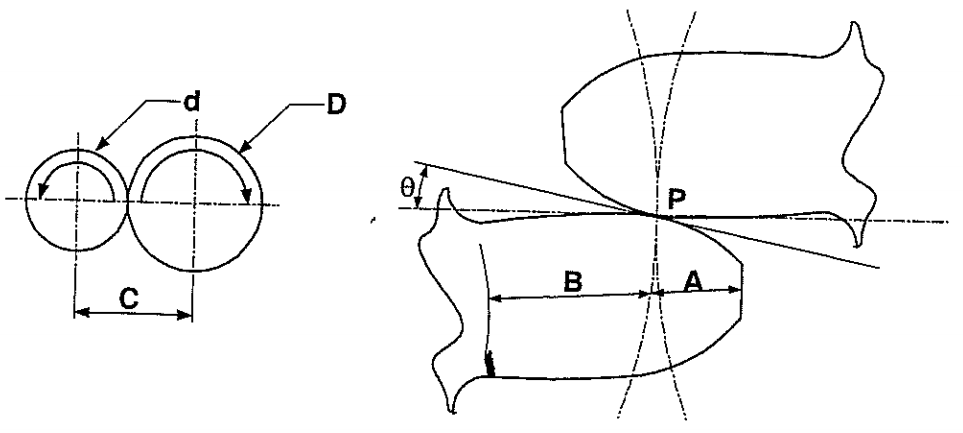
\includegraphics[width=0.9\textwidth]{figs/meshing-gears.png}
  \caption{Meshing gears}
  \label{fig-3}
\end{figure}

If the pinion has $n$ teeth and $\text{PCD}=d$, and the wheel has $N$ teeth and $\text{PCD}=D$ then:

\begin{equation}
  \text{VR} = \frac{N}{n} = \frac{D}{d}
\end{equation}

The nominal centre distance $C$ is:

\begin{equation}
  C = 0.5(d+D)
\end{equation}

This is known as the nominal centre distance because the actual centre distance is usually somewhat greater than this.

The height of a tooth above the PCD line is known as the addendum (A). The height of a tooth below the PCD line is known as the dedendum (B).

The angle made by the tangent to the gears at the point of contact is called the pressure angle ($\theta$). This angle is usually \ang{20} and should be assumed so unless otherwise stated.

The point of contact is called the pitch point (P). In order to obtain a constant velocity ratio the pitch point should not move as the gears move into and out of mesh. If the pitch point did move in and out with each mesh, then this would cause acceleration/deceleration with each mesh. If the gears are rotating at relatively high speeds this would cause high acceleration/deceleration with high inertia forces and accelerated wear.

The pitch point remains fixed when the gears are cut with an involute profile. The involute profile can best be demonstrated by unwinding a thin cord from around a cylinder as shown in Figure \ref{fig-4}.

\begin{figure}[h!]
  \center
  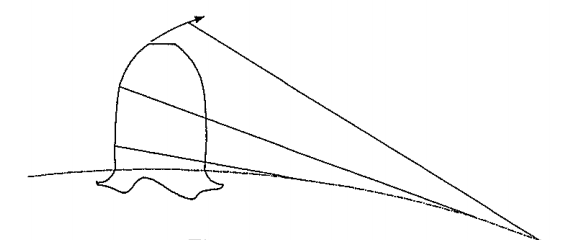
\includegraphics[width=0.9\textwidth]{figs/fig4.png}
  \caption{Involute profile}
  \label{fig-4}
\end{figure}

In\marginnote{Rack and Pinion} the case of a rack and pinion, the mating profile to the involute on the pinion is a straight sided rack as illustrated in \cref{fig-5}. The angle of the rack is the pressure angle as previously defined

\begin{figure}[h!]
  \center
  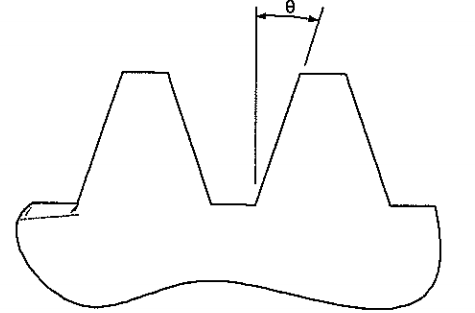
\includegraphics[width=0.8\textwidth]{figs/fig5.png}
  \caption{Rack profile}
  \label{fig-5}
\end{figure}

To\marginnote{Clearence} minimise friction, the teeth should contact only along the front face of the driver and the back face of the driven. There should be both circumferential and radial clearance as shown in \cref{fig-6}.

\begin{figure}[h!]
  \center
  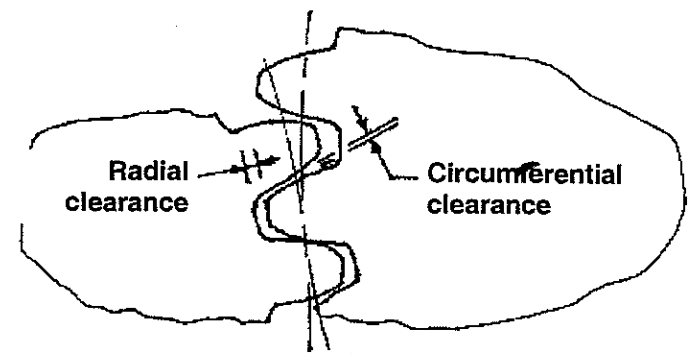
\includegraphics[width=0.9\textwidth]{figs/fig6.png}
  \caption{Clearence}
  \label{fig-6}
\end{figure}

Radial clearance (or bottom clearance) is obtained by making the dedendum greater than the addendum. Usually $\text{B}=1.25\text{A}$. Circumferential clearance is usually very small when the gears are new because wear automatically increases it. It can be obtained by making the centre distance slightly larger than the nominal centre distance. Circumferential clearance causes backlash and can be measured by holding one gear fixed and moving the other gear back and forth relative to it.

One\marginnote{Module (M)} of the most important parameters in gear design is the module which may be defined as the pitch circle diameter divided by the number of teeth. For a gear pair, the module must be the same for pinion and wheel. Hence:

\begin{equation}
  \text{M} = \frac{d}{n} = \frac{D}{N}
\end{equation}

Standard modules (first choice) in \si{\milli\metre} are:

1 1.25 1.5 2 2.5 3 4 5 6 8 10 12 16 20 25 32 40 50

As the module increases, the size of the gear teeth increase. That is, the gears become stronger and can transmit more torque and power. For example with a PCD of \SI{200}{\milli\metre}, a module of \SI{1}{\milli\metre} would mean 200 small teeth whereas a module of \SI{10}{\milli\metre} would mean 20 large teeth. This is illustrated in \cref{fig-7}.

\begin{figure}[h!]
  \center
  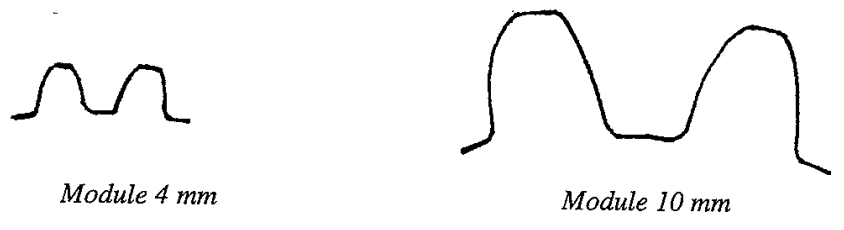
\includegraphics[width=0.9\textwidth]{figs/fig7.png}
  \caption{Module - tooth size comparison (PCD \SI{200}{\milli\metre})}
  \label{fig-7}
\end{figure}

The addendum, dedendum and depth of gear teeth are directly related to the module. For gear teeth of standard proportions the following relationships apply:

\begin{itemize}
  \item Addendum $\text{A} = \text{M}$
  \item Dedendum $\text{B} = 1.25\text{M}$
  \item Tooth depth $=\text{A}+\text{B}=2.25\text{M}$
\end{itemize}

The face width of gears is also related to the module but is also dependent upon the gear load (torque). The following rule-of-thumb face widths $\text{W}$ of the wheel are usual in mechanical power transmission:

\begin{itemize}
  \item Relatively light loads $\text{W}=8\text{M}$
  \item Moderate load $\text{W}=10\text{M}$
  \item Heavy loads $\text{W}=12\text{M}$
\end{itemize}

\textbf{Note:} The face width of the pinion is usually 5--10\% larger than the wheel (depending upon assembly tolerances)

A\marginnote{Example One} spur gear pair are to have a velocity reduction ratio in the range 2.5 to 2.7. The proposed number of teeth in the pinion is 18 with a module of 5mm. Determine:

\begin{enumerate}
  \item[a)] A suitable number of teeth in the wheel and the reduction ratio in order to have all hunting teeth,
  \item[b)] PCD of pinion and wheel,
  \item[c)] Nominal centre distance,
  \item[d)] Addendum, dedendum and tooth depth,
  \item[e)] Face width of pinion and wheel if loads can be described as moderate.
\end{enumerate}

a)\marginnote{Solution} Various combination of teeth in the wheel, velocity ratio and revolutions of the pinion when the cycle repeats are set out in the \cref{tbl-3}

\begin{table}[h]
  \caption{Pinion and wheel combinations}
  \label{tbl-3}
  \center
  \begin{tabular}{p{0.2\textwidth} p{0.2\textwidth} p{0.2\textwidth} p{0.24\textwidth}}
    \toprule
    Teeth in pinion & Teeth in wheel & Velocity Ratio & Pinion revolution when cycle repeats \\
    \midrule
    18 & 45 & 2.5 & 5 \\
    18 & 46 & 2.556 & 23 \\
    18 & 47 & 2.611 & 47 \\
    18 & 48 & 2.667 & 8 \\
    \bottomrule
  \end{tabular}
\end{table}

Hence it is seen that the only combination that give a velocity ratio in the required range with all teeth hunting is the 18:47 ratio. Hence choose \textbf{47} teeth in the wheel with velocity ratio \textbf{2.556}.

\noindent{} b)

\begin{itemize}
  \item PCD of the pinion $= 5 \times 18 = 90\si{\milli\metre}$
  \item PCD of the wheel $= 5 \times 47 = 235\si{\milli\metre}$
\end{itemize}

\noindent{} c) Nominal centre distance $C = 0.5(d+D) = 0.5(90+235)=162.5\si{\milli\metre}$

\noindent{} d)
\begin{itemize}
  \item Addendum $\text{A} = \text{M} = 5\si{\milli\metre}$
  \item Dedendum $\text{B} = 1.25\text{M} = 6.35\si{\milli\metre}$
  \item Tooth Depth $\text{A} + \text{B} = 11.25\si{\milli\metre}$
\end{itemize}

\noindent{} e)
\begin{itemize}
  \item For moderate loading assume face width of the wheel $\text{W}=10\text{M}=50\si{\milli\metre}$
  \item Face width of the pinion, say 7\% larger $= 1.07 \times 50 = 53.5\si{\milli\metre}$
\end{itemize}

\subsubsection{Gear design}

A comprehensive design procedure for gears is very complex and outside the scope of this manual. For example, AS2938 - Gears - Spur and Helical - Guide to Specification and Rating lists 88 different variables and constants and contains 32 different charts!

The most important factor to determine when designing gears for a certain application is the module. As has been stated, the greater the loading, the larger the size of the gear teeth and the larger the module.

A simplified factor to module selection is the use of a chart as the one given as \cref{fig-8}. This chart has been drawn for spur gears with face widths = 10M and with 18 teeth in the pinion. It may be used for face widths in the range 8-12M and for pinions with 17-19 teeth. It may also be used for helical angles up to \ang{20}. However, because helical gears are inherently stronger than spur gears, a somewhat smaller module will be satisfactory (say one standard size down).

\begin{figure}[th!]
  \center
  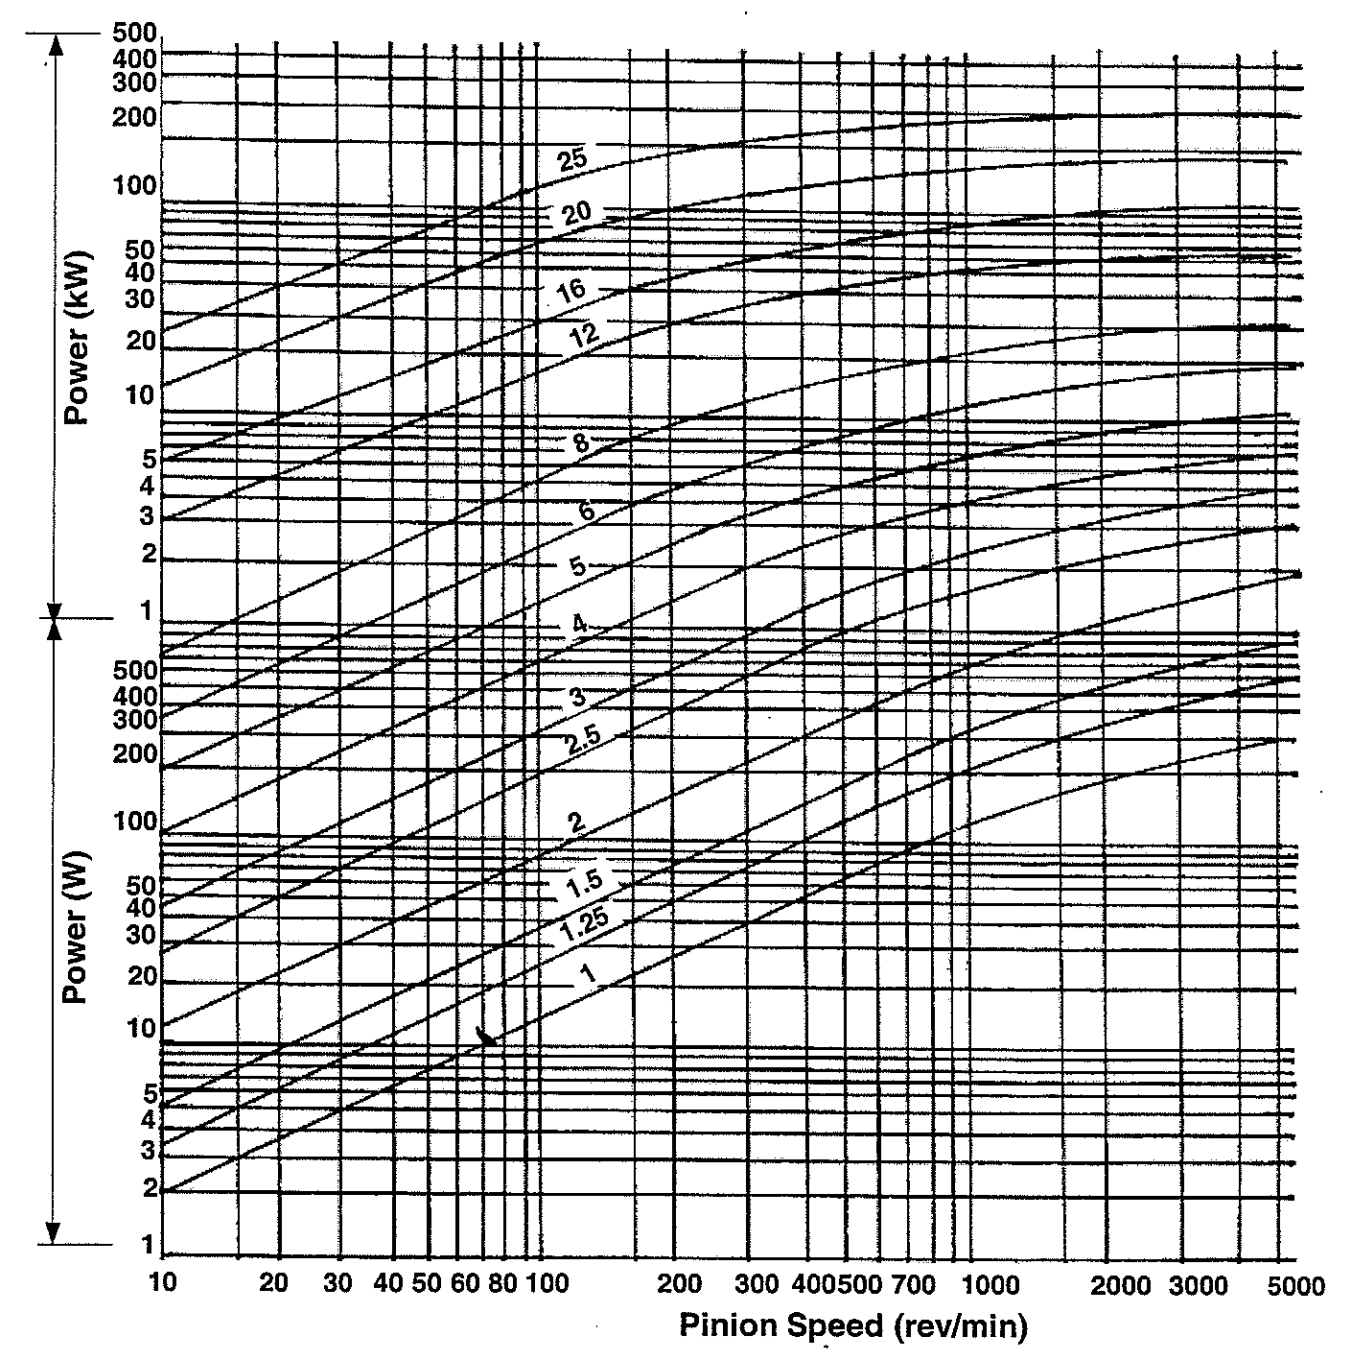
\includegraphics[width=0.9\textwidth]{figs/fig8.png}
  \caption{Module selection chart}
  \label{fig-8}
\end{figure}

A\marginnote{Example Two} helical pinion transmits \SI{20}{\kilo\watt} at \SI{1500}{rpm} to a mating gear. Loading is moderate. Determine suitable values for:

\begin{enumerate}
  \item[a)] The module for pinion and gear;
  \item[b)] The face width of the pinion and the gear;
  \item[c)] The PCD of the pinion.
\end{enumerate}

a)\marginnote{Solution} From \cref{fig-8}, the module lies between 6 and 8. A module of 7 is not standard (first choice). Because the gear is a helical one, the choice of the smaller module is justified. Hence choose $\text{M} = 6$.

b) With $\text{M}=6$ and face width of the gear $= 10 \text{M}$ (moderate loading), therefore the face width of the gear $= 60\si{\milli\metre}$.

For the pinion, make the face width about 7\% larger, say 64\si{\milli\metre}.

c) Make the number of teeth on the pinion = 19.

Then the pinion $\text{PCD} = 6 \times 19 =144\si{\milli\metre}$.

\subsubsection{Gear tooth forces}

The forces acting on gears in mesh occurs at the point of contact of the gears (the pitch point). The force $F$ as shown in \cref{fig-9}.

\begin{figure}[h!]
    \center
    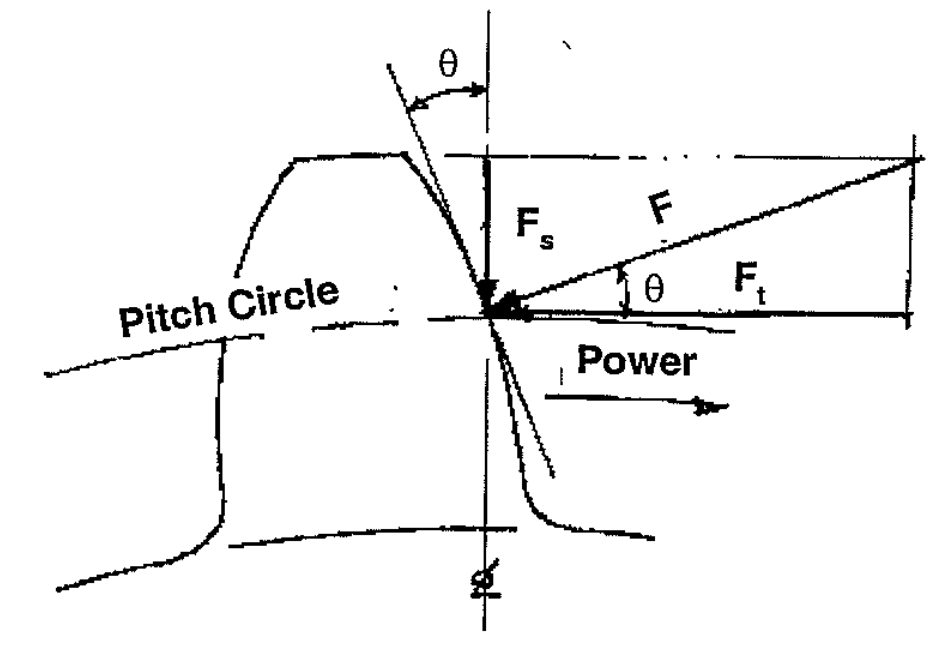
\includegraphics[width=0.9\textwidth]{figs/fig9.png}
    \caption{Module selection chart}
    \label{fig-9}
\end{figure}

In this diagram:

\begin{itemize}
  \item[$F=$] resultant transverse force on the tooth at the pitch point. This is also the resultant transverse load on the shaft at the location of the gear. Note that this force acts perpendicular to the tooth at the pitch point.
  \item[$F_s=$] separating (or radial) force on the tooth at the pitch point. Its line of action passes through the centrelines of the two gears. This force is needed to keep the gears together and without it, the gears would simply slip out of mesh and not transmit any torque.
  \item[$F_t=$] tangential force acting on the tooth at the pitch point. This force multiplied by the pitch circle radius gives the torque transmitted by the gear.
  \item[$\theta=$] the pressure angle, that is the angle between forces $F$ and $F_t$. For most gears, this angle is \ang{20} and should be assumed so unless otherwise stated.
\end{itemize}

Because\marginnote{Spur Gear Forces} torque is the tangential force multiplied by the pitch circle radius it is clear that the tangential force on the gear is calculated by:

\begin{equation}
  f_t = \frac{2T}{d}
\end{equation}

Where $T=$ Torque (\si{\newton\metre}) and $d=\text{PCD}$ of the gear in metres.

From \cref{fig-9}, the forces on the spur gear are as follows:

\marginnote{Separating Force}

\begin{equation}
  F_s = F_t\tan\theta
\end{equation}

\marginnote{Resultant Transverse Force}

\begin{equation}
  F=\sqrt{F_t^2+F_s^2}
\end{equation}

Because\marginnote{Helical Gear Forces} the teeth are cut at an angle (the helix angle), there is also an axial force on the gears. The tangential force is the same as for the spur gears but the formula for the separating force becomes:

\begin{equation}
  F_s = \frac{F_t\tan\theta}{\cos\alpha}
\end{equation}

Where $\alpha$ is the helix angle.

\marginnote{Axial Force}

\begin{equation}
  F_a = F_t\tan\alpha
\end{equation}

A\marginnote{Example Three} spur gear PCD \SI{100}{\milli\metre} transmits \SI{800}{\newton\metre} of torque. Determine the tangential, separating and resultant force on each gear.

The\marginnote{Solution} tangential force is:

\begin{equation}
  F_t = \frac{2T}{d} = \frac{2\times 800}{0.1} = 16\si{\kilo\newton}
\end{equation}

Assuming a pressure angle of \ang{20}, the separating force is:

\begin{equation}
  F_s = F_t\tan\theta = 16\tan20 = 5.82\si{\kilo\newton}
\end{equation}

The resultant force is:

\begin{equation}
  F = \sqrt{F_t^2+F_s^2} = \sqrt{16^2+5.82^2} = 17\si{\kilo\newton}
\end{equation}


Repeat\marginnote{Example Four} Example 3 for helical gears with helix angle \ang{20} (all other data being the same). Also calculate the axial force.

\begin{equation}
  F_t = \frac{2T}{d} = \frac{2\times 800}{0.1} = 16\si{\kilo\newton}
\end{equation}

\begin{equation}
  F_s = \frac{F_t\tan\theta}{\cos\alpha} = \frac{16\tan20}{\cos20} = 6.2\si{\kilo\newton}
\end{equation}

\begin{equation}
  F = \sqrt{F_t^2+F_s^2}=\sqrt{16^2+6.2^2}=17.2\si{\kilo\newton}
\end{equation}

\begin{equation}
  F_a = F_t\tan\alpha=16\tan20 = 5.82\si{\kilo\newton}
\end{equation}
